\documentclass[12pt,a4paper]{report}
\usepackage[utf8]{inputenc}
\usepackage[fleqn]{amsmath}
\usepackage{amsfonts}
\usepackage{amssymb}
\usepackage{graphicx}

\author{Kyle Swanson}
\title{Chapter 1 Exercises: Number Systems}
\setlength{\parindent}{0cm}

\begin{document}

\maketitle

\begin{normalsize}



\textbf{1.8} What is the largest 32-bit unsigned number?\\
$ 2^{32}-1 = 4,294,967,295$ \\

\textbf{1.10} What is the largest 32-bit binary number that can be represented with\\
(a) unsigned numbers?\\
$ 2^{32}-1 = 4,294,967,295 $

(b) two's complement numbers?\\
$ 2^{31}-1 = 2,147,483,647 $

(c) sign/magnitude numbers?\\
$ 2^{31}-1 = 2,147,483,647 $ \\

\textbf{1.12} What is the smallest (most negative) 32-bit binary number that can be represented with\\
(a) unsigned numbers?\\
If you can't have a sign, either it's impossible to have a negative value, or you assume that all values are negative. A negative-int data type I suppose.
$ -2^{32}-1 = -4,294,967,295 $

(b) two's complement numbers?\\
$ -2^{31} = -2,147,483,648 $

(c) sign/magnitude numbers?\\
$ -2^{31}-1 = -2,147,483,647 $ \\

\textbf{1.14} Convert the following unsigned binary numbers to decimal.\\
(a) $ 1110_{2} $ \\
$ 2^{3} + 2^{2} + 2^{1} + 0 = 14 $ \\
(b) $ 10 0100_{2} $ \\
$ 2^{5} + 2^{2} = 36 $ \\
(c) $ 1101 0111_{2} $ \\
$ 2^{7} + 2^{6} + 2^{4} + 2^{2} + 2^{1} + 2^{0} = 215 $ \\
(d) $ 011 1010 1010 0100_{2} $ \\
$ 2^{13} + 2^{12} + 2^{11} + 2^{9} + 2^{7} + 2^{5} + 2^{2} = 15,012 $ \\

\textbf{1.16} Repeat 1.14, but convert to hexadecimal. \\
Since they are split into 4 bit sections, just match each section with it's hex digit.\\
(a) $ 1110_{2} $ \\
$ 0xE $ \\
(b) $ 10\:0100_{2} $ \\
$ 0x24 $ \\
(c) $ 1101\:0111_{2} $ \\
$ 0xD7 $ \\
(d) $ 011\:1010\:1010\:0100_{2} $ \\
$ 0x3AA4 $ \\

\textbf{1.18} Convert the following hexadecimal numbers to decimal. \\
(a) $ 0x4E $ \\
$ 4*16^{1} + 14*16^{0} = 78 $ \\
(b) $ 0x7C $ \\
$ 7*16^{1} + 12*16^{0} = 124 $ \\
(c) $ 0xED3A $ \\
$ 14*16^{3} + 13*16^{2} + 3*16^{1} + 10*16^{0} = 60,730 $ \\
(d) $ 0x403FB001 $ \\
$ 4*16^{7} + 3*16^{5} + 15*16^{4} + 11*16^{3} + 1*16^{0} = 1,077,915,649 $ \\

\textbf{1.20} Repeat 1.18, but convert to unsigned binary. \\
Simply take each digit, and match it to it's binary equivalent. Then push the resulting sections together. \\
(a) $ 0x4E $ \\
$ 0100\: 1110 $ \\ \\
(b) $ 0x7C $ \\
$ 0111\: 1100 $ \\ \\
(c) $ 0xED3A $ \\
$ 1110\: 1101\: 0011\: 1010 $ \\ \\
(d) $ 0x403FB001 $ \\
$ 0100\: 0000\: 0011\: 1111\: 1011\: 0000\: 0000\: 0001 $ \\ \\

\textbf{1.22} Convert the following two's complement binary numbers to decimal. \\
(a) $ 1110_{2} $ \\ 
The left most bit is 1, flip the bits, $ 1110 = 0001 $ then add 1. $ 0001 + 0001 = 0010 = 2 $ \\
Since the left most bit was 1, the result is negative. $ -2 $ \\ \\
(b) $ 100011_{2} $ \\ 
$ 011100 + 000001 = 011101 $ \\
$ 2^{4} + 2^{3} + 2^{2} + 2^{0} = -29 $ \\ \\
(c) $ 01001110_{2} $ \\ 
The left most bit is 0, so this is a positive number. Continue as normal. \\
$ 2^{6} + 2^{3} + 2^{2} + 2^{1} = 78 $ \\ \\
(d) $ 10110101_{2} $ \\ 
$ 01001010 + 00000001 = 01001011 $ \\
$  2^{6} + 2^{3} + 2^{1} + 2^{0} = -75 $ \\ \\

\textbf{1.26} Convert the following decimal numbers to unsigned binary numbers. \\
(a) 14 \\
$ 14/2 = 7 r 0 $ \\
$ 7/2 = 3 r 1 $ \\
$ 3/2 = 1 r 1 $ \\
$ 1/2 = 0 r 1 $ \\
$ 14 = 1110 $ \\

(b) 52 \\
$ 52/2 = 26 r 0 $ \\
$ 26/2 = 13 r 0 $ \\
$ 13/2 = 6 r 1 $ \\
$ 6/2 = 3 r 0 $ \\
$ 3/2 = 1 r 1 $ \\
$ 1/2 = 0 r 1 $ \\
$ 52 = 110100 $ \\

(c) 339 \\
$ 339/2 = 169 r 1 $ \\
$ 169/2 = 84 r 1 $\\
$ 84/2 = 42 r 0 $\\
$ 42/2 = 21 r 0 $\\
$ 21/2 = 10 r 1 $\\
$ 10/2 = 5 r 0 $\\
$ 5/2 = 2 r 1 $\\
$ 2/2 = 1 r 0 $\\
$ 1/2 = 0 r 1 $\\
$ 339 = 101010011 $\\

(d) 711 \\
$ 711/2 = 355 r 1 $ \\
$ 355/2 = 177 r 1 $ \\
$ 177/2 = 88 r 1 $ \\
$ 88/2 = 44 r 0 $ \\
$ 44/2 = 22 r 0 $ \\
$ 22/2 = 11 r 0 $ \\
$ 11/2 = 5 r 1 $ \\
$ 5/2 = 2 r 1 $ \\
$ 2/2 = 1 r 0 $ \\
$ 1/2 = 0 r 1 $ \\
$ 711 = 1011000111 $ \\ 

\textbf{1.28} Repeat Exercise 1.26, but convert to hexadecimal. \\
Since it's converted to binary already, you can start with that, then go to hex. \\
(a) 14 \\
$ 14 = 1110 = 0xE $ \\

(b) 52 \\
$ 52 = 0011\: 0100 = 0x34$ \\

(c) 339 \\
$ 339 = 0001\: 0101\: 0011 = 0x153 $\\

(d) 711 \\
$ 711 = 0010\: 1100\: 0111 = 0x2C7 $ \\

\textbf{1.30} Convert the following decimal numbers to 8-bit two's complement numbers or indicate that the decimal number would overflow the range. \\
(a) 24 \\
$ 24/16 = 1r8 $ \\
$ 24 = 0x18 = 0001\: 1000 $ \\
Since it's positive, the leading bit should be 0. \\

(b) -59 \\
$ 59/16 = 3r11 $ \\
$ 59 = 0x3B = 0011\: 1011 $ \\
Invert bits and add 1 \\
$ 1100\: 0100 + 0001 = 1100\: 0101 $ \\

(c) 128 \\
$ 128/16 = 8r0 $ \\
$ 128 = 0x80 = 1000\: 0000 $ \\
But, we have a problem. Since 128 on it's own takes up 8 bits, this would read as $ -128 $ in two's complement. With only 8bits, there is no way to represent +128. \emph{Overflow} \\

(d) -150 \\
$ 150/16 = 9r6 $ \\
$ 150 = 0x96 = 1001\: 0110 $ \\
Invert and add 1, $ 0110\: 1001 + 0001 = 0110\: 1010 $ \\
Again, since we only have 8 bits, this causes an \emph{overflow}. \\

(e) 127 \\
$ 127/16 = 7r15 $ \\
$ 127 = 0x7F = 0111\: 1111 $ \\
Luckily, this does not overflow, but it is at the end of an 8bit two's complement numbers range. \\

\textbf{1.34} Convert the following 4-bit two's complement numbers to 8-bit two's complement numbers. \\
(a) 0111 \\
Since this is a positive number nothing needs to be changed. \\ 
$ 0000\: 0111 $ \\

(b) 1001 \\ 
Just add 1's to the bits in front, since this is a negative number. \\
$ 1111\: 1001 $ \\

\textbf{1.36} Repeat Exercise 1.34 if the numbers are unsigned rather than two's complement. \\
I'm not completely sure I understand this question. Are we converting two's complement numbers to 8bit unsigned? Or 4bit unsigned to 8bit two's complement? Or just unsigned to unsigned? \\
Either way, the answer should just be the original plus 0000 at the front. This is since, if they are unsigned to start with, they are positive, and therefore the two's will be positive. If they are two's moving to unsigned, \emph{b} just doesn't really make sense. Anyway, here's the answer assuming they are unsigned, moving to two's complement. \\ \\
(a) 0111 \\
$ 0000\: 0111 $ \\ \\
(b) 1001 \\
$ 0000\: 1001 $ \\

\textbf{1.38} Base 8 is referred to as octal. Convert each of the numbers from 1.26 to octal. \\
(a) 14 \\
$ 14/8 = 1r6 $ \\
$ 1/8 = 0r1 $ \\
$ 14 = 016 $ \\

(b) 52 \\
$ 52/8 = 6r4 $ \\
$ 6/8 = 0r6 $ \\
$ 52 = 064 $ \\

(c) 339 \\
$ 339/8 = 42r3 $ \\
$ 42/8 = 5r2 $ \\
$ 5/8 = 0r5 $ \\
$ 339 = 0523 $ \\

(d) 711 \\
$ 711/8 = 88r7 $ \\
$ 88/8 = 11r0 $ \\
$ 11/8 = 1r3 $ \\
$ 1/8 = 0r1 $ \\
$ 711 = 01307 $ \\

\textbf{1.40} Convert each of the following octal numbers to binary, hexadecimal, and decimal. \\
In the following questions, converting to binary, then binary to hex is easiest. \\

(a) 023 \\
binary: $ 010\: 011 $ \\
hex: $ 0x13 $ \\
decimal: $ 2*8^{1} + 3*8^{0} = 19 $ \\

(b) 045 \\
binary: $ 100\: 101 $ \\
hex: $ 0x25 $ \\
decimal: $ 4*8^{1} + 5*8^{0} = 37 $ \\

(c) 0371 \\
binary: $ 011\: 111\: 001 $ \\
hex: $ 0\: 1111\: 1001\: = 0xF9 $ \\
decimal: $ 3*8^{2} + 7*8^{1} + 1*8^{0} = 249 $ \\

(d) 02560 \\
binary: $ 010\: 101\: 110\: 000 $ \\
hex: $ 0101\: 0111\: 0000 = 0x570 $ \\
decimal: $ 2*8^{3} + 5*8^{2} + 6*8^{1} + 0*8^{0} = 1392 $ \\

\textbf{1.42} How many 7-bit two's complement numbers are greater than 0? How many numbers are less than 0 \\
The range of a 7-bit two's complement number is 
$ -(2^{6})\: to\: 2^{6}-1 $, which is $ -64\: to\: 63 $ \\
So the number \textbf{greater} than 0, is 63, and the number \textbf{less} is 64. \\

\textbf{1.44} How many bytes are in a 64-bit word? \\
8-bits to one byte. Therefore, $ 64/8 = 8\: bytes $ \\

\textbf{1.50} Draw a line number analogous to Figure 1.11 for 3-bit unsigned, two's complement, and sign/magnitude numbers. \\
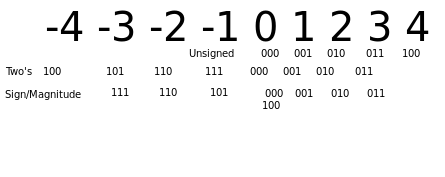
\includegraphics[scale=0.8]{Number_line.png} 

\textbf{1.52} Perform the following additions of unsigned binary numbers. Indicate whether or not the sum overflows a 4-bit result. \\
(a) $ 1011 + 0100 $ \\
$ 1111 $ \\

(b) $ 1101 + 1011 $ \\
\begin{tabular}{c@{\,}c@{\,}c@{\,}c@{\,}c}
  & 1 & 1 & 1 & \\
  & 1 & 1 & 0 & 1 \\
+ & 1 & 0 & 1 & 1 \\
\hline
1 & 1 & 0 & 0 & 0 \\
\end{tabular} \\
This does \emph{overflow} the 4-bit result. The 4-bit version would simply be $ 1000 $ \\

\textbf{1.54} Repeat exercise 1.52, assuming that the binary numbers are in two's complement form. \\
(a) $ 1011 + 0100 $ \\
$ 1011 = -5 $ \\
$ 0100 = 4 $ \\
$ 1011 + 0100 = 1111 = -1 $ \\

(b) $ 1101 + 1011 $ \\
$ 1101 = -3 $ \\
$ 1011 = -5 $ \\
\begin{tabular}{c@{\,}c@{\,}c@{\,}c@{\,}c}
  & 1 & 1 & 1 & \\
  & 1 & 1 & 0 & 1 \\
+ & 1 & 0 & 1 & 1 \\
\hline
1 & 1 & 0 & 0 & 0 \\
\end{tabular} \\
The far left bit is lost, but it isn't needed in this instance, $ 1000 = -8 $, so the answer is still correct. \\

\textbf{1.56} Convert the following decimal numbers to 6-bit two's complement binary numbers and add them. Indicate whether or not the sum overflows a 6-bit result. \\
(a) 16 + 9 \\
$ 16 = 010000 $ \\
$ 9 = 001001 $ \\
$ 010000 + 001001 = 011001 $ \\
Does not overflow \\

(b) 27 + 31 \\
$ 27/2 = 13r1 $ \\
$ 13/2 = 6r1 $ \\
$ 6/2 = 3r0 $ \\
$ 3/2 = 1r1 $ \\
$ 1/2 = 0r1 $ \\
$ 27 = 011011 $ \\
$ 31/2 = 15r1 $ \\
$ 15/2 = 7r1 $ \\
$ 7/2 = 3r1 $ \\
$ 3/2 = 1r1 $ \\
$ 1/2 = 0r1 $ \\
$ 31 = 011111 $ \\ \\
\begin{tabular}{c@{\,}c@{\,}c@{\,}c@{\,}c@{\,}c@{\,}c}
  & 1 & 1 & 1 & 1 & 1 & \\
  & 0 & 1 & 1 & 0 & 1 & 1 \\
+ & 0 & 1 & 1 & 1 & 1 & 1 \\
\hline
  & 1 & 1 & 1 & 0 & 1 & 0 \\
\end{tabular} \\
$ 111010 = -6 $ \\
Overflows. Even though there are no lost bits, since they msb is set to 1, with not enough bits for a leading 0. This is represented as a -6, which is incorrect. \\

(c) -4 + 19 \\
$ -4 = 000100 = 111011 + 0001 = 111100 $ \\
$ 19/2 = 9r1 $ \\
$ 9/2 = 4r1 $ \\
$ 4/2 = 2r0 $ \\
$ 2/2 = 1r0 $ \\
$ 1/2 = 0r1$ \\
$ 19 = 010011 $ \\ 
\begin{tabular}{c@{\,}c@{\,}c@{\,}c@{\,}c@{\,}c@{\,}c}
1 & 1 &   &   &   &   & \\
  & 1 & 1 & 1 & 1 & 0 & 0 \\
+ & 0 & 1 & 0 & 0 & 1 & 1 \\
\hline
1 & 0 & 0 & 1 & 1 & 1 & 1 \\
\end{tabular} \\
No overflow, since -4 + 19 is a positive number, the msb should be 0. \\
$ 001111 = 15 $ \\

(d) 3 + -32 \\
$ 3 = 000011 $ \\
$ -32 = 100000 $ \\
$ 000011 + 100000 = 100011 = -29 $ \\
Does not overflow \\

(e) -16 + -9 \\
$ -16 = 010000 = 101111 + 0001 = 110000 $ \\
$ -9 = 001001 = 110110 + 0001 = 110111 $ \\
$ 110000 + 110111 = 1\: 100111 $ \\
$ 100111 = -25 $, one extra bit is tossed out, but it isn't needed. \\
Does not overflow \\

(f) -27 + -31 \\
$ 27 = 011011 = 100101 = -27 $ \\
$ 31 = 011111 = 100001 = -31 $ \\ 
$ 100101 + 100001 = 000110 = 6 $ \\
This overflows, it would need 7-bits to properly represent -58. \\

\textbf{1.58} Perform the following additions of unsigned hexadecimal numbers. Indicate whether or not the sum overflows an 8bit (two hex digit) result. \\
(a) 0x7 + 0x9 \\
\begin{tabular}{c@{\,}c@{\,}c@{\,}c}
  & & 1 &     \\
  & &   & 7 \\
+ & &   & 9 \\
\hline
  & & 1 & 0 \\
\end{tabular} \\
0x10 \\
Does not overflow. \\

(b) 0x13 + 0x28 \\
\begin{tabular}{c@{\,}c@{\,}c@{\,}c}
  & &   &     \\
  & & 1 & 3 \\
+ & & 2 & 8 \\
\hline
  & & 3 & B \\
\end{tabular} \\
0x3B \\
Does not overflow \\

(c) 0xAB + 0x3E \\
\begin{tabular}{c@{\,}c@{\,}c@{\,}c}
  & & 1 &     \\
  & & A & B \\
+ & & 3 & E \\
\hline
  & & E & 9 \\
\end{tabular} \\
0xE9 \\
Does not overflow \\

(d) 0x8F + 0xAD \\
\begin{tabular}{c@{\,}c@{\,}c@{\,}c}
  & 1 & 1 &     \\
  &  & A & D \\
+ &  & 8 & F \\
\hline
  & 1 & 3 & C \\
\end{tabular} \\
0x13C \\
Overflows \\

\textbf{1.60} Convert the following decimal numbers to 5-bit two's complement binary numbers and subtract them. Indicate whether or not the difference overflows a 5-bit result. \\
(a) 9 - 7 \\
$ 9 = 01001 $ \\
$ 7 = 00111 $ \\
$ -7 = 11000 + 00001 = 11001 $ \\
\begin{tabular}{c@{\,}c@{\,}c@{\,}c@{\,}c@{\,}c}
1 & 1 &   &   & 1 & \\
  & 0 & 1 & 0 & 0 & 1 \\
+ & 1 & 1 & 0 & 0 & 1 \\
\hline
1 & 0 & 0 & 0 & 1 & 0 \\
\end{tabular} \\
Does not overflow \\
$ 100010 = 2 $ \\

(b) 12 -15 \\
$ 12 = 01100 $ \\
$ 15 = 01111 $ \\
$ -15 = 10001 $ \\
\begin{tabular}{c@{\,}c@{\,}c@{\,}c@{\,}c@{\,}c}
  &   &   &   &   & \\
  & 0 & 1 & 1 & 0 & 0 \\
+ & 1 & 0 & 0 & 0 & 1 \\
\hline
  & 1 & 1 & 1 & 0 & 1 \\
\end{tabular} \\
Does not overflow \\
$ 11101 = -3 $ \\

(c) -6 - 11 \\
$ 6 = 00110 $ \\
$ -6 = 11010 $ \\
$ 11 = 01011 $ \\
$ -11 = 10101 $ \\
\begin{tabular}{c@{\,}c@{\,}c@{\,}c@{\,}c@{\,}c}
1 &   &   &   &   & \\
  & 1 & 1 & 0 & 1 & 0 \\
+ & 1 & 0 & 1 & 0 & 1 \\
\hline
1 & 0 & 1 & 1 & 1 & 1 \\
\end{tabular} \\
This overflows, it also gives an incorrect result. Since -6 - 11 requires more than 5 bits. \\
$ 01111 = 15 $ \\

(d) 4 -- 8 \\
$ 4 = 00100 $ \\
$ 8 = 01000 $ \\
$ -8 = 11000 $ \\
\begin{tabular}{c@{\,}c@{\,}c@{\,}c@{\,}c@{\,}c}
  &   &   &   &   & \\
  & 0 & 0 & 1 & 0 & 0 \\
+ & 0 & 1 & 0 & 0 & 0 \\
\hline
  & 0 & 1 & 1 & 0 & 0 \\
\end{tabular} \\
Does not overflow \\
$ 01100 = 12 $ \\

\textbf{1.65} Answer the following questions related to \textit{Binary Coded Decimal} systems. \\
(a) Write 371 in BCD \\
$ 3 = 0011 $ \\
$ 7 = 0111 $ \\
$ 1 = 0001 $ \\
$ 001101110001 $ \\ 

(b) Convert $ 000110000111_{BCD} $ to decimal. \\
$ 0001 = 1 $ \\
$ 1000 = 8 $ \\
$ 0111 = 7 $ \\
$ 000110000111 = 187 $ \\

(c) Convert $ 10010101_{BCD} $ to binary \\
$ 1001 = 9 $ \\
$ 0101 = 5 $ \\
$ 95/2 = 47r1 $ \\
$ 47/2 = 23r1 $ \\
$ 23/2 = 11r1 $ \\
$ 11/2 = 5r1 $ \\
$ 5/2 = 2r1 $ \\
$ 2/2 = 1r0 $ \\
$ 1/2 = 0r1 $ \\
$ 95 = 1011111 $ \\

(d) Explain the disadvantage of BCD when compared to binary representation of numbers. \\
It takes more bits to store the same number. \\
Take the example above. 95 in binary requires 7 bits, where the BCD version requires 8. \\
8 bits in BCD only get you up to 99. But 8 bits with binary can get you all the way to 255. \\

\end{normalsize}

\end{document}